\documentclass{article}
\usepackage{preamble}
\title{The Dudley Co\"{o}p Points Chart Overview}
\author{Ben Whitney}
\date{2013-08-07}
\begin{document}

\thispagestyle{empty}
\begin{center}
{
\LARGE
\scshape
The Dudley Co\"{o}p\\
Points Chart Overview
}


\includegraphics[width=0.6\textwidth]{images/greenie_meanies.jpg}

{
\Large
Ben Whitney\\
\href{mailto:ben.e.whitney@post.harvard.edu}{\texttt ben.e.whitney@post.harvard.edu}\\
Summer 2013
}
\end{center}
\newpage

\tableofcontents

\section{The Basics}
Some of the effort required to keep the house running takes the form of chores.
Over the course of a semester we aim for an equal division of this work among the co\"{o}pers.
To say that one co\"{o}per's share is ``(un)equal" to another's, we must have a way to measure (collections of) chores.
This metric we use for this purpose is points.
Every chore has a point value, which is mostly (but only mostly) based on how long it takes to do.
A typical chore gets you 3--4 points per hour of work, but the rate for a particular chore might be twice or half that, depending on desireability, any flexibility in when it can be done, co\"{o}p priorities, etc.
Neither point values nor the chores themselves are set in stone, and every co\"{o}p should feel comfortable tweaking and experimenting to find a mix that is fair and works.
The remaining hurdle is selecting the specific chores that will make up a co\"{o}per's share.
To simplify this process, the semester is split into two-week cycles.
Each cycle contains daily, weekly, and biweekly chores, plus any special tasks that might be needed.
The Points Steward keeps track of all the chores in a cycle and sums their point values to find a total number of points to be done in that cycle.
This total is divided by the number of co\"{o}pers, producing the individual points load (not account for stewardships) for that cycle.\footnote{%
See Section~\ref{subsec:calculationOfLoads} for a full explanation of how loads are calculated.%
}
Co\"{o}pers then sign themselves up chores so that they're doing as many points as they owe.
This is done using the points chart.

\section{Using the Points Chart}
It will be easier to understand this section if you have the chart open in front of you.

\subsection{Signing Up and Off}
We used to sign up for points on a physical chart, but now we use a Google Spreadsheet.
A few days before the start of a new cycle, the Points Steward will send an email to the co\"{o}p list asking everyone to begin signing up for their points. Upon opening the chart, you will see a sheet entitled `Summary' that lists two balances for each co\"{o}per.
The first step to using the chart is understanding what is meant by these balances.

\begin{description}
\item[Current Balance]
The total point value of the chores you've signed up for in the current cycle minus your load for the cycle.
If your balance is positive, you've signed up for too many chores; if it's negative, you've signed up for too few.
The goal, of course, is to have it near zero (near is good enough).
\item[Previous Balance]
The total point value of the chore you \emph{did} (not signed up for) in the previous cycle minus your load for that cycle.
Again, the goal balance is zero, but this might not be possible depending on how many chores you signed up for.
\end{description}


Based on these balances, you will sign up for (or remove yourself from\footnote{%
If you are doing this during (as opposed to before) the actual cycle, you \emph{need} to email the list telling people you're dropping the chore.%
}%
) chores.
To do this, write your initials in the sign up slot of the chore on the `Chart' sheet for the cycle.
A picture works better than words here, so go look at the chart.


How does the chart determine how many chores you did in a cycle?
A chore is considered completed only if someone \emph{other than you} signs off on it.
This is done by simply typing their initials under your name on the chart.
People commonly forget this step.
If your Previous Balance is high, it's probably because you have lots of chores that haven't been signed off on!

The name you use to sign up for chores and the initials you use to sign off on chores should be entered in the `Settings' sheet.
They must be unique (although names and initials may overlap).
The chart will recognize your name and initials no matter which case you use, creates another restriction: two names or two sets of initials may not differ only by the cases of the letter (`ABC' and `AbC' are treated in the same way by the chart).
One value, `void' is off-limits.
If either the sign up cell or the sign off cell of a chore has value `void' (or `vOId,' etc.), the chart considers the chore not to have been done.
The person who signed up for it will get no points for it, and its value will be subtracted from the total sum billed to the co\"{o}p for that cycle.

\subsection{Absences and Loans}
If you are away from the co\"{o}p, you can get your load reduced (to be proportional to the time you are here) by reporting yourself absent.
To do this, click on the `Co-op' menu item and then select `Report an absence.'

You can also get your load reduced if for whatever reason you are going to have a difficult time completing your normal amount of chores. 
For this, click on the `Co-op' menu item and then select `Take or repay a loan.'
In contrast to absences, loans are handled internally as simple point amounts that are added to our subtracted from your load for the cycle.
The chart will keep track of the loans you've taken so you know how much to pay back later on.

Loans are most often used by seniors writing theses.
However, I want to emphasize that all co\"{o}pers should feel encouraged to ask for a loan if they need it.
Depression, injury, a horrible series of midterms, or a difficult breakup are all perfectly good reasons to take a lower load.
And finally, if you realize you're going to have trouble making up those points, just talk to the Points Steward (or the Presidents, or tutors, or Karen Flood).
The Points Steward only wants the house to run well and for people to do a fair amount of chores.
We're not a bank.  

\subsection{Extras}
We will now discuss the remaining entries of the `Co-op' menu item.

\begin{description}
\item[Send a reminder]
You will write a little message and this function will text it to the person signed up for the chore you've selected.
If a sign up cell isn't selected, the function will complain and tell you what you've done wrong.
\item[Add chores to Google Calendar]
This function finds all the chore you've signed up for in the current cycle and adds them to your Google Calendar in a calendar called `Co-op Chores.'
There is some customization you can do in terms of what kinds of reminders you get and how often before the start of the chore they come.
\item[Add co\"{o}pers to Google Contacts]
This function creates a co\"{o}p group in your Contacts and adds everyone to it.
It does this using the `Contact Info' page.
\end{description}


For the second and third of these to work, you must be logged into a Google Account when running them.
To emphasize, the chores and contacts are both created in new groups, so that your main calendar/contact list isn't polluted and you can easily undo whatever changes the functions make.

There is one more big extra, but it is not listed in `Co-op.'
Go back to the `Settings' sheet and look at the columns asking whether you want email and text reminders.
You can already get email and text reminders by adding your chores to Google Calendar, but this is done separately, by the chart itself.
There is less customizability with this method, since all your chores for the day will be lumped into one email/text in the morning, not sent close to the time of the chore.
However, some people have found the reminders useful in addition to or instead of using GCal, so the feature remains.

\section{The Stewardship}
This section covers \emph{only} the aspects of the stewardship relating to running the chart, and it assumes more familiarity with the system.

\subsection{The Calculation of Loads}\label{subsec:calculationOfLoads}
It is important to understand where loads come from even if you never need to do any of the math yourself.
The formula used is
\begin{equation*}
\frac{\text{TCP} + \text{TSP} + \text{TCS} + \text{TL}}{\text{TDI}}\text{CDI} - (\text{CSC} + \text{CPB} + \text{CSP} + \text{CL})
\end{equation*}
where we've abbreviated
\begin{center}
\begin{tabular}{llll}
TCP  & Total Chore Points             &
CSC  & Co\"{o}per's Stewardship Credit\\
TSP  & Total Special Points           &
CPB  & Co\"{o}per's Previous Balance\\
TSC  & Total Stewardship Credits      &
CSP  & Co\"{o}per's Special Points\\
TL   & Total Loans                    &
CL   & Co\"{o}per's Loan\\
TDI  & Total Days In                  &
CDI  & Co\"{o}per's Days In
\end{tabular}
\end{center}
The fraction represents rate of points per co\"{o}per-day (analogous to man-hour) that needs to be achieved for all the cycle's work to be completed.
Total Days In is the number of co\"{o}per-days available to the co\"{o}p, and is found by summing Co\"{o}per's Days In over all the co\"{o}pers.
Each resident co\"{o}per contributes 14 per cycle, unless they are absent, in which the value will be however many days they are in the co\"{o}p. 
Quarterboarders contribute 3.5 co\"{o}per-days (a quarter of 14), which should also be changed to be proportional to their time in Cambridge if case of absence.

The numerator should evaluate to the total number of points that need doing.
The first three terms fit cleanly into this, but Total Loans requires some explaining.
When a co\"{o}per takes a loan, no points are created or destroyed.
They just do fewer chores, and the rest of us pick up the slack.
Following this intuition, we previously handled loans internally as absences, i.e. reductions to Co\"{o}per's Days In.
This would reduce Total Days In, increasing the points per co\"{o}per-day fraction, and so increase the loads of everyone (including the loan-taker).
All the chores would still get done.

Now loans are handled more like an invisible, custom chore that the loan-taker does and is credited for before the start of the cycle. 
Having done this `chore,' the loan-taker signs up for fewer normal chores, and so of course the rest of the co\"{o}p makes up the difference. 
This is achieved by adding the sum of all the loans to the chore points, special points, and stewardship credits totals.

The fraction is scaled by the co\"{o}per-days for the person in question to get a basic load, which can then be changed by the sum on the right.
Perhaps the most important of these terms is Co\"{o}per's Previous Balance.
This term ensures that surpluses and deficits carried over from the previous cycle affect the current load.
The other terms are included because people expect their loads to be the number of chores they need to sign up for, not the sum total of all co\"{o}p work expected of them this cycle.
So, any stewardships, special points, and loans are factored in here, leaving only the load, which the whole formula evaluates to.

\subsection{Changing the Chart}
With so many tasks accomplished with scripts, you might worry you will break the chart if you change anything.
The script does pull all its data from the chart, so there is a real possibility of breaking things, but it is also written to seamlessly handle common changes.
First, a rule:
\begin{center}
If you're making significant changes to the chart, {\scshape make a backup!}
\end{center}
By `significant changes' I mean things like rewriting script functions, totally reformatting the `Chart' sheets, and doing anything that might result in the loss of sign up/off data.
Shuffling around columns, fiddling with formulae, and changing the information on the `Summary' sheet are examples of things that are fine doing on the live chart.
Finally, note that changes to some of the core areas of the chart, such as the contact information, may require a rebuilding of \texttt{PSEUDO\_GLOBALS} object (see Subsection \ref{subsec:pseudoGlobals}).

\subsubsection{Changing the Roster}
To add a new co\"{o}per or quarterboarder, first add an entry for them in the `Basic Data' sheet.
The `Contact Info' and `Settings' sheets' `Co-oper' columns are linked to the `Basic Data' sheet, so this should result in entries on those sheets.
Fill the entries in.
Note that either appending the new entry at the bottom or inserting it somewhere in the middle (say to preserve alphabetical ordering) is fine.
Just check at the end that `Basic Data,' `Contact Info,' and `Settings' use the same order.
Also follow this rule when changing the name (`Co-oper' entry) of a co\"{o}per.

Next, make sure the co\"{o}per appears in \emph{every} `Loads' sheet.
For cycles before they joined, you can mark them down as absent for 14 days, and then they should accrue no loads.
Finally, fiddle with the `Summary' sheet to make sure the new co\"{o}per's data is being shown.
You might have to shuffle the entries around a little to make sure everything still looks nice (this is assuming you’re still using the three-column format it has now).

\subsubsection{Changing Chores}
Adding a new chore requires a little less work, although you still have to be careful.
First, make a `Chart' sheet entry in an open space (or replace an old chore).
After modifying the `Chart' sheets, make entries on the corresponding `Point Values' sheets.
The points value of the chore should go in the sign up cell.
For daily chores \emph{except Kitchen Deep Clean chores} (that is, MCU 1--MCU 2 at the time of this writing), the chore name should go over in the first column.
For all other chores, it should go in the cell immediately above the point value.
Follow the example of other chores.

Next go to the `Basic Data' sheet and enter the chore's name in the `Chore Name' column.
The start time should be in 24-hour time notation (e.g.~18:00 for 6 {\scshape pm}) and the duration should be in minutes.
The day offset is how many days after the chore's date the chore should be done.
For example, MCU 2 on Wednesday should be done early Thursday morning, so its day offset is 1.
For chores that should happen before the chore's day, use a negative number.
For how exactly a chore's date is determined, read the code for \texttt{\_SignUpCell}.


What if there wasn't enough open space on the chart to put your chore?
Or maybe you are trying to create a new daily chore?
In this case, you are free to insert rows as you please, but there is a little extra work to be done.
Open the script editor and find the definitions of \texttt{DAILY\_CHORES\_ROWS} and \texttt{WEEKLY\_CHORES\_ROWS}.
Make changes such that daily chores (currently MCU 1--MCU 2 plus all Kitchen Deep Clean chores) have their rows found in the former, and that all weekly chores (currently Miscellaneous and Bathrooms) have their rows found in the latter.
The distinction between daily and weekly chores is used in determining when to send out reminders, with both the \texttt{sendReminders} and
\texttt{addToGoogleCalendar} functions.

Finally, there is one more thing to check.
As we mentioned above, some chores need their name entered immediately above the sign up cell (on the `Points Value' chart), while others have theirs stored in the first column, and the distinction is not cleanly daily chores versus weekly chores.
When adding chores on new rows, make sure that the choreName property definition in the \texttt{\_SignUpCell} constructor is going to behave properly.
The code is pretty simple but I fear confusing the reader, so I will let you figure it out yourselves or contact me for an explanation.

To delete a chore, remove it from the `Chart' sheet(s) and zero out the point value on the corresponding `Point Values' sheet(s).
Feel free to delete the entries on the `Points Values' and `Basic Data' sheets, but this is not strictly necessary.

\subsection{Miscellaneous Tips}
\begin{itemize}
\item
Special points are useful both for one-off chores and when two people split the work of a chore.
or example, if person A does half of person B's DRP, increase person A's special points by 2 and decrease person B's special points by 2.
\item
If you or other co\"{o}pers find the `Summary' sheet confusing, feel free to change it.
The notion of `balances' is important for how the chart keeps track of loads behind the scenes, but some other way of presenting the numbers might be clearer.
For an example I used for a semester, see Figure \ref{fig:example}.

\begin{figure}[h]
\centering
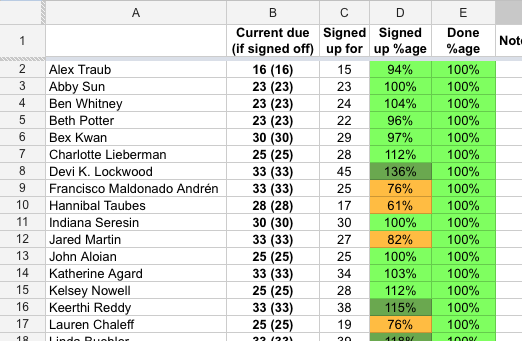
\includegraphics[width=0.6\textwidth]{images/alternate_summary}
\caption{%
Another way to display loads.
The `if signed off' number was used to signal if a co\"{o}per's load was high because of chores from the previous cycle that weren't signed off on.%
}
\label{fig:example}
\end{figure}

\item 
Doing some basic diagnostics on the `Loads' sheet can help you spot problems.
The sum of all current balances and the sum of all previous balances both should always be 0.
Common culprits here include chore that haven't been signed up for for the current balances and chores that haven't been signed off on/voided for previous balances.
The sum of the `Current signed up' column should equal the `Sum of Chore Points' cell, etc.
\item
Encourage co\"{o}pers to come to you with questions.
Doing some detective work to solve problems will increase your understanding of the system and help you find any bugs or errors.
You will get your share of people complaining that their load is too high when they haven't been doing their chores, though.
\item
When making new sheets or using the \texttt{propagateSheetChanges} function, make sure all the formula references are pointing to the right sheets.
\end{itemize}

\section{Script Documentation}
The goal of this section is that reading it will make you sufficiently well-versed in the objects and methods that the chart uses that you will be able to troubleshoot any problems that come up and implement any features you want to add.
The script is written in Google Apps Script, which is something like JavaScript 1.8 with JavaScript 1.6 syntax and access to a lot of Google APIs.

\begin{center}
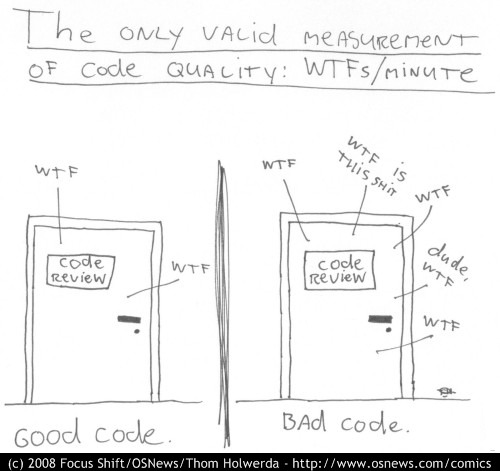
\includegraphics[width=0.6\textwidth]{images/wtfm}
\end{center}

\subsection{Pseudo-Globals}\label{subsec:pseudoGlobals}
I would guess that the first question to spring into your mind while reading the script would be what the role of the \texttt{PSEUDO\_GLOBALS} object constructed/fetched at the start the big functions is.
(If some other question came first, email me so I can get better at coding and stop doing bizarre things.)
What distinguishes the contents of \texttt{PSEUDO\_GLOBALS} and the actual global objects, \texttt{UI\_BUILDERS} and \texttt{POINTS\_UTILITIES}?
The key difference is that the latter two require no calls to any Google services and so are cheap to build.
\texttt{PSEUDO\_GLOBALS} contains the commonly used spreadsheet data, which is expensive to fetch.
It also contains plenty of cheaply made objects (e.g. \texttt{DAILY\_CHORES\_ROWS} and the \texttt{\_Cooper} constructor); these are included partly for simplicity and in some cases to avoid thorny scope issues.

So why separate out all the time-consuming stuff if you're just going to build them at the beginning of most functions?
The answer lies in how UiApp, a service I've used to create user interfaces, processes user input.
When a SubmitButton is pressed (inside a FormPanel), the \texttt{doPost} function is executed.
\emph{But it is executed inside a brand new instance!}
All the `global' code is rerun, but any changes made to those values are not kept.
Unfortunately I do not have a source backing up this assertion; it is the result of a lot of hours spent reading StackOverflow questions and dealing with baffling errors.
Two problems result:
\begin{enumerate}
\item
When \texttt{doPost} is entered, global variables need to be recalculated.
If these recalculations involve service (SpreadsheetApp, MailApp, ScriptDb, etc.) calls or any other time-consuming code, this
will decrease the responsiveness of the UI.\footnote{%
I’m not positive the effect is noticeable.
I think it is, though, and in any case this way is more efficient.%
}
These globals are not needed inside \texttt{doPost}, so we can do without them.
\item
\texttt{doPost} needs to return the UI Application that called it in order for it to be completely closed, but we also need to communicate the information the user has entered into the UI.
This cannot be done by saving it to a global variable, for the reasons mentioned above.
So, it must be saved inside doPost to something that separate `instances' of the script can access.
The choices I've encountered are
\begin{description}
\item[ScriptDb]
The first implementation used ScriptDb.
Unfortunately, there is an unresolved bug with the database where it will report containing key/value pairs but will not spit them out.
This option is off the table until that is resolved.
\item[CacheService]
This replaced ScriptDb.
So far using a private cache has been working well, but Google is not entirely clear on whether we should consider the cache a completely safe place to store data (at least before it is set to expire).
\item[SpreadsheetApp]
Writing values to the spreadsheet is (or at least has been in the past) faster than storing them with ScriptDb.
JIf CacheService fails, we should can use this, but it is an ugly solution to me.
\end{description}
\end{enumerate}
\texttt{PSEUDO\_GLOBALS} is (almost) the output of \texttt{pseudoGlobalsBuiler}, as the name suggests.
New functions should instead define it as the output of \texttt{pseudoGlobalsFetcher} (as is done currently), since this function looks first in the public cache for a saved version of the pseudo-global objects.
Presumably this is faster than redefining them.
Additionally, \texttt{pseudoGlobalsFetcher} redefines the time-sensitive objects (e.g. \texttt{currentCycle}).
In some scenarios, such as when a quarterboarder has their contact information added, the other `static' objects of \texttt{PSEUDO\_GLOBALS} may become outdated.
To remedy this, simply remove it from the public cache; it will be rebuilt when next \texttt{pseudoGlobalsFetcher} is called.

Finally, be warned that I made a lot of these decisions using rules of thumb, not any rigorous profiling.
I'm sorry if that's not what you wanted to hear just now!

\subsection{User Interfaces}
Building user interfaces using UiApp has been frustrating, involving a lot of guesswork and the occasional Google bug that needed to be sidestepped (I'm thinking of problems in capturing which RadioButton is selected).
If you need to make a new interface, hopefully your experience can be made smoother by following the examples contained in \texttt{UI\_BUILDERS}, which contains both the functions that create UIs and a \texttt{DEFAULTS} object that contains some lengths I tried to use consistently.
If your UI just needs to display a message, take a look at \texttt{UI\_BUILDERS.displayMessage} or maybe \texttt{UI\_BUILDERS.displayMessageAndLink}.
Otherwise, you will need to capture some user input.
The way I have done this is to enclose all the widgets in a FormPanel that includes a SubmitButton (or multiple SubmitButtons, as used in \texttt{UI\_BUILDERS.getLoanInfo}).
When the SubmitButton is clicked, \texttt{doPost} is called with an argument containing the submission event information.

There can be only one \texttt{doPost} function in the script, so we have to include some logic to handle the different requirements of each UI.
One option would be to write a very simple \texttt{doPost} function and leave the processing to the normal functions (like \texttt{userInitiatedReminder}) that called the UI building function.
Here is such a \texttt{doPost} function using CacheService:
\begin{minted}{js}
function doPost(e) {
  var privateCache = CacheService.getPrivateCache();
  privateCache.put('userResponses', Utilities.jsonStringify(e.parameter), 60);
  var currentApp = UiApp.getActiveApplication();
  currentApp.close();
  return currentApp;
}
\end{minted}
Instead of this approach, what I have done is include all the logic inside \texttt{doPost}, using a switch on the value of \texttt{e.parameter.identifier}.
So, each UI builder has a hidden TextBox named \texttt{identifier} whose value is some unique string that corresponds to some post-processing commands in \texttt{doPost}.

If you are ambitious, feel free to rewrite \texttt{UI\_BUILDERS} using HtmlService, which is apparently more powerful than UiApp.

\subsection{Points Utilities}
Most of the members of the \texttt{POINTS\_UTILITIES} object are simple functions that do various things to arrays of arrays and arrays of more general objects.
The exceptions are \texttt{retrieveRange} and \texttt{retrieveSheet}, used in reading or writing data to the spreadsheet, and \texttt{waitForUIResponse}, whose utility is less obvious.
As it turns out, \emph{function execution does not pause after a UI is displayed}.
Left to its own devices, the computer\footnote{% 
Now seems as good a time as any to mention that the script is executed server-side.
The only exception I know of is ClientHandlers, which we do use in some places.%
}
will barrel on without the user input, typically resulting in an error.
So, we need insert a pause and continue only after the user has submitted the information we need.
\texttt{waitForUIResponse} achieves this purpose.
At this time it is written for CacheService storage.
If in the future ScriptDb, SpreadsheetApp, or some other service is used to pass values from the main script instance to the one where \texttt{doPost} runs, make sure that the storage medium is cleared before the waiting begins, because otherwise \texttt{waitForUIResponse} will find the old user responses immediately, leaving no time for the user to submit their own.

\subsection{The Rest}
Rather than comprehensively review the remaining functions, I will leave some miscellaneous tips/thoughts
here and try to comment the code helpfully.
\begin{itemize}
\item
\texttt{processAbsence} overwrites the absence amount for the chosen cycle, while \texttt{processLoan} adds to the current amount.
\item
The total loan balance written by \texttt{processLoan} could be replaced by a function adding the loan balances for each cycle.
It might be better if this was a `spreadsheet function' rather than a `script function' because it would involve pulling cells from each of the `Loads' sheets, which might take some time.
Maybe it would be negligible, though.
\item
You will save yourself a lot of effort if you learn to use the \texttt{allCoopers}, \texttt{cycleSignUpCells}, and \texttt{daySignUpCells} quasi-iterators found in \texttt{PSEUDO\_GLOBALS}.
I call them `quasi-iterators' because Google Apps Script doesn't seem to support real custom iterators, as JavaScript 1.8 does.
You can use them similarly to how you use query results from ScriptDb, with \texttt{hasNext} and \texttt{next} methods.
\item
After using \texttt{propagateSheetChanges}, you'll have to go through the sheets and change any references to previous sheets (for example in the `Previous balance' column of `Loads' sheets).
And {\scshape be careful} when using this function, as it deletes sheets!
\item
The script editor debugger and Logger don't work sometimes.
It seems to happen whenever they're used inside \texttt{doPost}, but I've seen the problem occur even when all the code is being
executed in one `instance.'
To deal with this, I would often use a quick little function like the following:
\begin{minted}{js}
function grossLog(message, location) {
  var PSEUDO_GLOBALS = pseudoGlobalsFetcher();
  var logRange = PSEUDO_GLOBALS.SPREADSHEET.getSheetByName('Contact Info')
  .getRange(location)
  logRange.setValue(logRange.getValue()+'\n'+message);
}
\end{minted}
\item
Please update and comment the code if you have anything to add! I would be grateful for another person's perspective.
If you'd like to get more involved, I'll probably be putting this all up on GitHub and you can fork the repository.
\item
\href{mailto:ben.e.whitney@post.harvard.edu}{Email me} with any and all questions.
I can probably save you a lot of time.
Good luck!
\end{itemize}
\end{document}
